\documentclass[openany]{book}

\usepackage[margin=1in]{geometry}
\usepackage{amsmath,amsfonts,amsthm, amssymb}
\usepackage{yhmath}
\usepackage{mathrsfs}
\usepackage{mathtools}
\usepackage{xcolor}
\usepackage{graphicx}
\usepackage{comment}
\usepackage{tikz-cd}
\usepackage{quiver}
\renewcommand{\familydefault}{ppl}
\newcommand{\tr}{\text{tr}}
\newcommand{\R}{\mathbb{R}}
\newcommand{\E}{\mathbb{E}}
\newcommand{\Z}{\mathbb{Z}}
\newcommand{\C}{\mathbb{C}}
\newcommand{\F}{\mathbb{F}}
\newcommand{\la}{\langle}
\newcommand{\ra}{\rangle}
\newcommand{\colim}{\text{colim}}
\DeclareMathOperator{\im}{im}
\let\oldemptyset\emptyset
\let\emptyset\varnothing
\newcommand{\tor}{\text{Tor}}
\newcommand{\id}{\text{id}}
\newcommand{\ext}{\text{Ext}}
\newcommand{\ptop}{\text{PTop}}
\newcommand{\pt}{\text{pt}}
\newcommand{\ach}{\text{Ach}}
\newcommand{\Q}{\mathbb{Q}}
\newcommand{\gal}{\text{Gal}}
\newcommand{\diverg}{\operatorname{div}}
\newcommand{\curl}{\operatorname{curl}}
\usepackage{pgfplots}
\pgfplotsset{compat=newest}

\usepackage{thmtools,thm-restate}

% Fixing mdframed skip below
% See https://tex.stackexchange.com/a/292090/143086
\usepackage[framemethod=TikZ]{mdframed}
\usepackage{xpatch}
\makeatletter
\xpatchcmd{\endmdframed}
	{\aftergroup\endmdf@trivlist\color@endgroup}
	{\endmdf@trivlist\color@endgroup\@doendpe}
	{}{}
\makeatother

\definecolor{huilightpink}{HTML}{fcf2f9}
\definecolor{huidarkpink}{HTML}{ed34b3}
\declaretheoremstyle[
	mdframed={
		backgroundcolor=huilightpink,
		linecolor=huidarkpink,
		rightline=false,
		topline=false,
		bottomline=false,
		linewidth=2pt,
		innertopmargin=5pt,
		innerbottommargin=8pt,
		innerleftmargin=8pt,
		leftmargin=-2pt,
		skipbelow=2pt,
		nobreak
	},
	headfont=\normalfont\bfseries\color{huidarkpink}
]{huipinkbox}
\declaretheorem[style=huipinkbox,name=Theorem,within=chapter]{thm}
\declaretheorem[style=huipinkbox,name=Theorem,sibling=thm]{theorem}





\definecolor{huilightyellow}{HTML}{fff5d6}
\definecolor{huidarkyellow}{HTML}{fcad03}
\declaretheoremstyle[
	mdframed={
		backgroundcolor=huilightyellow,
		linecolor=huidarkyellow,
		rightline=false,
		topline=false,
		bottomline=false,
		linewidth=2pt,
		innertopmargin=5pt,
		innerbottommargin=8pt,
		innerleftmargin=8pt,
		leftmargin=-2pt,
		skipbelow=2pt,
		nobreak
	},
	headfont=\normalfont\bfseries\color{huidarkyellow}
]{huiyellowbox}
\declaretheorem[style=huiyellowbox,name=Proposition,within=chapter]{prop}

\definecolor{huilightpurple}{HTML}{faf2ff}
\definecolor{huidarkpurple}{HTML}{912ed9}
\declaretheoremstyle[
	mdframed={
		backgroundcolor=huilightpurple,
		linecolor=huidarkpurple,
		rightline=false,
		topline=false,
		bottomline=false,
		linewidth=2pt,
		innertopmargin=5pt,
		innerbottommargin=8pt,
		innerleftmargin=8pt,
		leftmargin=-2pt,
		skipbelow=2pt,
		nobreak
	},
	headfont=\normalfont\bfseries\color{huidarkpurple}
]{huipurplebox}
\declaretheorem[style=huipurplebox,name=Lemma,within=chapter]{lem}


\definecolor{huilightpurple}{HTML}{faf2ff}
\definecolor{huidarkpurple}{HTML}{912ed9}
\declaretheoremstyle[
	mdframed={
		backgroundcolor=huilightpurple,
		linecolor=huidarkpurple,
		rightline=false,
		topline=false,
		bottomline=false,
		linewidth=2pt,
		innertopmargin=5pt,
		innerbottommargin=8pt,
		innerleftmargin=8pt,
		leftmargin=-2pt,
		skipbelow=2pt,
		nobreak
	},
	headfont=\normalfont\bfseries\color{huidarkpurple}
]{huipurplebox}
\declaretheorem[style=huipurplebox,name=Definition,within=chapter]{defn}

\definecolor{huilightblue}{HTML}{edf9ff}
\definecolor{huidarkblue}{HTML}{4b79db}
\declaretheoremstyle[
	mdframed={
		backgroundcolor=huilightblue,
		linecolor=huidarkblue,
		rightline=false,
		topline=false,
		bottomline=false,
		linewidth=2pt,
		innertopmargin=5pt,
		innerbottommargin=8pt,
		innerleftmargin=8pt,
		leftmargin=-2pt,
		skipbelow=2pt,
		nobreak
	},
	headfont=\normalfont\bfseries\color{huidarkblue}
]{huiblueblox}
\declaretheorem[style=huiblueblox,name=Example,within=chapter]{example}

\declaretheoremstyle[
	mdframed={
		backgroundcolor=huilightblue,
		linecolor=huidarkblue,
		rightline=false,
		topline=false,
		bottomline=false,
		linewidth=2pt,
		innertopmargin=5pt,
		innerbottommargin=8pt,
		innerleftmargin=8pt,
		leftmargin=-2pt,
		skipbelow=2pt,
		nobreak
	},
	headfont=\normalfont\bfseries\color{huidarkblue}
]{huiblueblox}
\declaretheorem[style=huiblueblox,name=Problem,within=chapter]{prob}

\newcommand{\nirwarnsymbol}{%
	
\begin{tikzpicture}[baseline=(x.base)]
		\draw[rounded corners=.01em] (-.05em,-1.07em)rectangle(.05em,.78em);
		\draw[fill=white,rounded corners=1.3] (0,.75em)--(.75em,0)--(0,-.75em)--(-.75em,0)--cycle;
		\draw[line width=0.2mm, line cap=round](-.4em,-1.07em)--(.4em,-1.07em);
		\node(x) at (0,0em) {};
		% Thank you https://tex.stackexchange.com/a/262510
		\draw[
			line cap=but,
			line join=round,
			x=.5em,
			line width=0.5mm,
			y=1*(height("Z")-\pgflinewidth)*(1-sin(10)),
			rotate=-10,
			rounded corners=1.5pt,
		](-0.57, 0.57) -- (0.57, 0.57) -- (-0.57, -0.57) -- (0.57, -0.57);
	\end{tikzpicture}%
}

%%%%%%%%%%%%%%%%%%%%%%%%%%%%%%%%%%%%%%%%%%%% MARGINS
\usepackage{marginnote}
% Thank you https://tex.stackexchange.com/a/472882
% Makes marginnotes always appear on the left, apparently
%
\makeatletter
\long\def\@mn@@@marginnote[#1]#2[#3]{%
	\begingroup
		\ifmmode\mn@strut\let\@tempa\mn@vadjust\else
			\if@inlabel\leavevmode\fi
			\ifhmode\mn@strut\let\@tempa\mn@vadjust\else\let\@tempa\mn@vlap\fi
		\fi
		\@tempa{%
			\vbox to\z@{%
				\vss
				\@mn@margintest
				\if@reversemargin\if@tempswa
						\@tempswafalse
					\else
						\@tempswatrue
				\fi\fi

					\llap{%
						\vbox to\z@{\kern\marginnotevadjust\kern #3
							\vbox to\z@{%
								\hsize\marginparwidth
								\linewidth\hsize
								\kern-\parskip
								%\mn@parboxrestore
								\marginfont\raggedleftmarginnote\strut\hspace{\z@}%
								\ignorespaces#1\endgraf
								\vss
							}%
							\vss
						}%
						\if@mn@verbose
							\PackageInfo{marginnote}{xpos seems to be \@mn@currxpos}%
						\fi
						\begingroup
							\ifx\@mn@currxpos\relax\else\ifx\@mn@currpos\@empty\else
									\kern\@mn@currxpos
							\fi\fi
							\ifx\@mn@currpage\relax
								\let\@mn@currpage\@ne
							\fi
							\if@twoside\ifodd\@mn@currpage\relax
									\kern-\oddsidemargin
								\else
									\kern-\evensidemargin
								\fi
							\else
								\kern-\oddsidemargin
							\fi
							\kern-1in
						\endgroup
						\kern\marginparsep
					}%
			}%
		}%
	\endgroup
}
\makeatother
%
% Mostly for todonotes
\renewcommand{\marginpar}{\marginnote}
%%%%%%%%%%%%%%%%%%%%%%%%%%%%%%%%%%%%%%%%%%%% /MARGINS

\definecolor{nirlightred}{RGB}{250, 220, 220}
\definecolor{nirdarkred}{HTML}{f40000}
\declaretheoremstyle[
	mdframed={
		backgroundcolor=nirlightred,
		linecolor=nirdarkred,
		rightline=false,
		topline=false,
		bottomline=false,
		linewidth=2pt,
		innertopmargin=5pt,
		innerbottommargin=8pt,
		innerleftmargin=8pt,
		leftmargin=-2pt,
		skipbelow=2pt,
		nobreak
	},
	headfont=\normalfont\bfseries\color{nirdarkred}
]{nirredbox}

% \makeatletter
% \declaretheorem[
% 	style=nirredbox,
% 	name=Warning,
% 	sibling=thm,
% 	% without \leavevmode, the first item in a list gets misformatted
% 	postheadhook={\leavevmode\marginnote{\nirwarnsymbol}[-3pt]%
% 	\ifthmt@thisistheone% restatable makes alignment weird
% 		\hspace{-2.2pt}%
% 	\fi}
% ]{warn}
% \makeatother

\newcommand{\nirideasymbol}{%
	
\begin{tikzpicture}[baseline=(x.base)]
		\draw[rounded corners=.01em] (-.05em,-1.07em)rectangle(.05em,.78em);
		\draw[fill=white,rounded corners=1.3] (0,.75em)--(.75em,0)--(0,-.75em)--(-.75em,0)--cycle;
		\draw[line width=0.2mm, line cap=round](-.4em,-1.07em)--(.4em,-1.07em);
		\node(x) at (0,0em) {};
		\node at (0,0em) {{\textbf{!}}};
	\end{tikzpicture}%
}
\renewcommand{\nirwarnsymbol}{%
	
\begin{tikzpicture}[baseline=(x.base)]
		\draw[rounded corners=.01em] (-.05em,-1.07em)rectangle(.05em,.78em);
		\draw[fill=white,rounded corners=1.3] (0,.75em)--(.75em,0)--(0,-.75em)--(-.75em,0)--cycle;
		\draw[line width=0.2mm, line cap=round](-.4em,-1.07em)--(.4em,-1.07em);
		\node(x) at (0,0em) {};
		% Thank you https://tex.stackexchange.com/a/262510
		\draw[
			line cap=but,
			line join=round,
			x=.5em,
			line width=0.5mm,
			y=1*(height("Z")-\pgflinewidth)*(1-sin(10)),
			rotate=-10,
			rounded corners=1.5pt,
		](-0.57, 0.57) -- (0.57, 0.57) -- (-0.57, -0.57) -- (0.57, -0.57);
	\end{tikzpicture}%
}
\makeatletter
\declaretheorem[
	style=nirredbox,
	name=Idea,
	sibling=thm,
	% without \leavevmode, the first item in a list gets misformatted
	postheadhook={\leavevmode\marginnote{\nirideasymbol}[-3pt]%
	\ifthmt@thisistheone% restatable makes alignment weird
		\hspace{-2.2pt}%
	\fi}
]{idea}

\declaretheorem[
	style=nirredbox,
	name=Warning,
	sibling=thm,
	% without \leavevmode, the first item in a list gets misformatted
	postheadhook={\leavevmode\marginnote{\nirwarnsymbol}[-3pt]%
	\ifthmt@thisistheone% restatable makes alignment weird
		\hspace{-2.2pt}%
	\fi}
]{warn}
\makeatother

\title{Calc III Sections
\\ 
\vspace{0.4cm}
\large Fall 2025}






\date{\today}
\author{Hui Sun}


\begin{document}

\maketitle

% \tableofcontents
\newpage


\begin{center}
    \Large Calc III-Week 12 (11/10-14)
\end{center}

\renewcommand\thesection{\arabic{section}}

\noindent






\begin{defn}[path integral]
    Let $c:[a,b]\to\R^3$ be a path of $C^1$ and $f:\R^3\to\R$ is such that $f\circ c$ is continuous on $[a,b]$, The \textbf{path integral} of $f(x,y,z)$ along the path $c$ is given by 
    \begin{align*}
        \int_c fds&=\int_a^bf(c(t))\|c'(t)\|dt\\
        &=\int_a^bf(x(t),y(t), z(t))\|c'(t)\|dt
    \end{align*}
\end{defn}



\begin{defn}[line integral]
    Let $F$ be a vector field on $\R^3$ that is continuous on the $C^1$ path $c:[a,b]\to\R^3$, where $c(t)=(x(t), y(t), z(t))$. We define $\int_c F\cdot ds$, the \textbf{line integral} of $F$ along $c$ by the following
    \begin{align*}
        \int_c F\cdot ds&=\int_a^bF(c(t))\cdot c'(t)dt\\
        &=\int_a^b \left(F_1\frac{dx}{dt}+F_2\frac{dy}{dt}+F_3\frac{dz}{dt}\right)dt\\
        &\coloneq\int_c F_1dx+F_2dy+F_3dz
    \end{align*}
    the expression $F_1dx+F_2dy+F_3dz$ is called the \textbf{differential form}.
\end{defn}

% \begin{defn}[differential form]
%     We also write the line integral above as 
%     \begin{equation*}
%         \int_cF\cdot ds=\int_c F_1dx+F_2dy+F_3dz
%     \end{equation*}
%     where $F=(F_1,F_2,F_3)$. 
% \end{defn}

\begin{example}[work done along a path]
    The force field $F$ on a particle moving along a path $c:[a,b]\to\R^3$ is given by 
    \begin{equation*}
        \text{ work done by } F=\int_a^bF(c(t))\cdot c'(t)dt
    \end{equation*}
\end{example}

\begin{defn}[reparametrization]
    Let $h: I\to I_1$ be a $C^1$ real-valued bijective function. Let $c: I_1\to\R^3$ be a piecewise $C^1$ path. Then we call the composition 
    \begin{equation*}
        p=c\circ h: I\to\R^3
    \end{equation*}
    a \textbf{ reparametrization} of $c$.
\end{defn}

\begin{example}
    Let $c:[0,1]\to\R^3$ be a $C^1$ path, then consider $h: [0,1]\to [0,1]$, where $h(t)=1-t$. Then the path 
    \begin{equation*}
        c_{\text{op}}=c\circ h(t)=c(1-t)
    \end{equation*}
    is the same path in the opposite direction.
\end{example}

\begin{prop}[reparametrization for path integrals]
    Let $c$ be a $C^1$ path and $c'$ be any reparametrization of $c$, and let $f$ be a continuous function on the image of $c$, then 
    \begin{equation*}
        \int_cf(x,y,z)ds=\int_{c'}f(x,y,z)ds
    \end{equation*}
\end{prop}

\begin{prop}[reparametrization for line integrals]
    Let $F$ be a vector feld continuous on the $C^1$ path $c:[a,b]\to\R^3$, and let $c':[a',b']\to\R^3$ be a reparametrization of $c$. If $c'$ is orientation-preserving, then 
    \begin{equation*}
        \int_{c'}F\cdot ds=\int_c F\cdot ds
    \end{equation*}
    If $c'$ is orientation-reversing, then 
    \begin{equation*}
        \int_{c'}F\cdot ds=-\int_cF\cdot ds
    \end{equation*}
\end{prop}

\begin{prop}[fundamental theorem of line integrals]
    Suppose $f:\R^3\to\R$ is of $C^1$ and that $c:[a,b]\to\R^3$ is piecewise $C^1$. Then 
    \begin{equation*}
        \int_c\nabla f\cdot ds=f(c(b))-f(c(a))
    \end{equation*}
\end{prop}

\begin{prob}
    Let $c:[a,b]\to\R^3$ be a $C^1$ path, find a reparametrization $\tilde{c}=c\circ h$, such that $\tilde{c}:[0,1]\to\R^3$.
\end{prob}
\begin{proof}
    Define $h(t)=a+(b-a)t$, where $0\leq t\leq 1$.
\end{proof}


\begin{prob}
    Suppose that $\nabla f(x,y,z)=(2x^2, y, -z)$, and that $f(0,1,-1)=2$. What is the value of $f(2, 1, 1)$?
\end{prob}
\begin{proof}
    By the fundamental theorem of line integrals, we know 
    \begin{align*}
        f(2,1,1)&=\int_\ell \nabla f \cdot ds+f(0,1,-1)\\
        &=\int_0^1 \nabla f(2t, 1, 2t-1)\cdot (2,0, 2)dt+f(0,1,-1)\\
        &=\int_0^1 \left(16t^2+2-4t\right)dt+2\\
        &=\frac{22}{3}
    \end{align*}
\end{proof}

\begin{prob}
    Compute the path integral of $f(x,y,z)=2x+y-z$ over the curve $c$, where $c$ is the intersection of the two surfaces below:
    \begin{equation*}
        y=x, \quad y^2+z^2=4
    \end{equation*}
    Hint: first find a parametrization of $c$, then use the formula of path integral.
\end{prob}
\begin{proof}
    Using polar coordinates, we can write $y=2\cos\theta, z=2\sin\theta$, and since $y=x$, we know $x=2\cos\theta$, thus the parametrization is given by 
    \begin{equation*}
        (2\cos\theta, 2\cos\theta, r\sin\theta), \quad 0\leq \theta\leq 2\pi
    \end{equation*}
    Now 
    \begin{equation*}
        \int_0^{2\pi}2(2\cos t)+2\cos t-2\sin tdt=0
    \end{equation*}
\end{proof}

\begin{prob}
    Suppose path $c$ has length $l$, and $F$ is a vector field such that $\|F\|\leq M$. Prove that 
    \begin{equation*}
        \left|\int_c F\cdot ds\right|\leq Ml
    \end{equation*}
    (Hint: Cauchy-Schwarz.)
\end{prob}
\begin{proof}
    \begin{align*}
        \left|\int_cF\cdot ds\right|&=\left|\int_a^b F(c(t))\cdot c'(t)dt\right|\\
        &\leq\int_a^b\left|F(c(t))\cdot c'(t)\right|dt\\
        &\leq\int_a^b\|F(c(t))\|\cdot\|c'(t)\|dt\\
        &\leq Ml
    \end{align*}
\end{proof}


\begin{prob}[Group work]
    Given vector field $F(x,y)=(1,1)$, and the following heart is given by the parametrization:
    \begin{equation*}
        c(t)=((1-\sin t)\cos t, (1-\sin t)\sin t) \quad \text{ where } 0\leq t\leq 2\pi
    \end{equation*}
    Group 1: what is the work done by going up the top of the heart? ($0\leq t\leq \pi$).
    
    \noindent
    Group 2: what is the work done by going up the bottom of the heart? ($\pi\leq t\leq 2\pi$).
    \begin{center}
    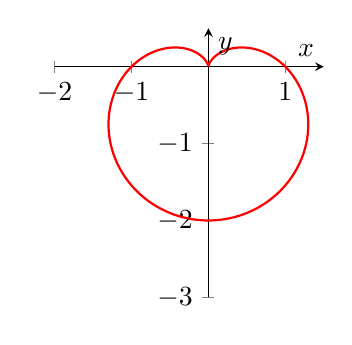
\begin{tikzpicture}
        \begin{axis}[
            axis lines = middle,
            xlabel = \(x\),
            ylabel = \(y\),
            xmin = -2, xmax = 1.5,
            ymin = -3, ymax = 0.5,
            width = 5cm,
            height = 5cm,
            trig format plots=rad % Use radians for trigonometric functions
          ]
          \addplot [
              domain = 0:2*pi,
              samples = 200,
              smooth,
              thick,
              red
            ] ({(1 - sin(x)) * cos(x)}, {(1 - sin(x)) * sin(x)});
        \end{axis}
      \end{tikzpicture}
    \end{center}
\end{prob}
\begin{proof}
    No need to actually compute $c'(t)$! For Group 1, we see that 
    \begin{align*}
        \int_0^\pi F(c(t))\cdot c'(t)dt&=\int_0^\pi x'(t)+y'(t)dt \tag{$c(t)=(x(t),y(t))$}\\
        &=x(\pi)+y(\pi)-x(0)-y(0)\\
        &=-2
    \end{align*}
    Similarly, 
    \begin{equation*}
        \int_{\pi}^{2\pi}F(c(t))\cdot c'(t)dt=2
    \end{equation*}
    Thus combined 
    \begin{equation*}
        \int_0^{2\pi}F(c(t))\cdot c'(t)dt=0
    \end{equation*}
\end{proof}


















\end{document}